
%(BEGIN_QUESTION)
% Copyright 2011, Tony R. Kuphaldt, released under the Creative Commons Attribution License (v 1.0)
% This means you may do almost anything with this work of mine, so long as you give me proper credit

Temperature control in this multi-bed chemical reactor is quite critical.  The chemical reaction happening inside of it is {\it exothermic}, which means it gives off heat.  If any of the catalyst beds inside the reactor gets too hot, the reaction could ``run away'' and destroy the catalyst:

$$\includegraphics[width=15.5cm]{i02467x01.eps}$$

Explain how the selector functions improve the safety and reliability of the control system for this reactor.  In particular, explain why {\it median-select} functions are used at each of the catalyst beds, and why a {\it high-select} function is used before the temperature controller.

\vskip 20pt \vbox{\hrule \hbox{\strut \vrule{} {\bf Suggestions for Socratic discussion} \vrule} \hrule}

\begin{itemize}
\item{} For those who have studied chemistry, what is a {\it catalyst} used for in chemical reaction engineering?
\item{} What is a {\it PSV}, and what is one doing in this process?
\item{} Predict the effects resulting from one of the transmitters in this system failing with either a {\it high} or a {\it low} signal.
\item{} Modify the control strategy (and the piping if necessary) to permit individual temperature control of each catalyst bed inside the reactor.
\end{itemize}

\underbar{file i02467}
%(END_QUESTION)





%(BEGIN_ANSWER)


%(END_ANSWER)





%(BEGIN_NOTES)

\vfil \eject

\noindent
{\bf Prep Quiz:}

A chemical reaction process that is {\it exothermic} generally needs what kind of temperature control system?

\begin{itemize}
\item{} A system to control the amount of {\it heating fluid} sent to the reactor
\vskip 5pt 
\item{} An air-operated control valve that is fail-closed (not fail-open!)
\vskip 5pt 
\item{} A system to control the amount of {\it steam} sent to the reactor
\vskip 5pt 
\item{} A temperature controller cascaded to one or more flow controllers
\vskip 5pt 
\item{} A system using type K thermocouples as the primary sensing elements
\vskip 5pt 
\item{} A system to control the amount of {\it coolant} sent to the reactor
\end{itemize}

%INDEX% Relay, computational: selector functions
%INDEX% Safety, redundancy: analog voting
%INDEX% Safety, redundancy: multiple transmitters

%(END_NOTES)


